\section{654 --- Maximum Binary Tree}
Given an integer array with no duplicates. A maximum tree building on this array is defined as follow:

\begin{itemize}
\item The root is the maximum number in the array.
\item The left subtree is the maximum tree constructed from left part subarray divided by the maximum number.
\item The right subtree is the maximum tree constructed from right part subarray divided by the maximum number.

\end{itemize}
Construct the maximum tree by the given array and output the root node of this tree.

\paragraph{Example 1:}

\begin{flushleft}
\textbf{Input}: \lstinline[language=C++, basicstyle=\small\ttfamily, keywordstyle=\bfseries\color{green!40!black}]|[3,2,1,6,0,5]|

\textbf{Output}: return the tree root node representing the following tree:

\begin{figure}[H]
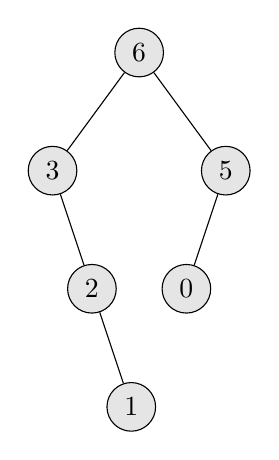
\begin{tikzpicture}
[every node/.style={draw, circle, fill=gray!20!, minimum size=5mm},
level 1/.style={sibling distance=22mm},
level 2/.style={sibling distance=10mm}]
\node{6}
child{node{3} child[missing] child{node{2} child[missing] child{node{1}}}}
child{node{5} child{node{0}} child[missing]};
\end{tikzpicture}
\end{figure}
\end{flushleft}

\paragraph{Note:}

\begin{itemize}
\item The size of the given array will be in the range \lstinline[language=Java, basicstyle=\small\ttfamily, keywordstyle=\bfseries\color{green!40!black}]|[1,1000]|.
\end{itemize}

\subsection{Divide And Conquer}
Divide the array into two halves per the maximum element. Recursively calling build function to create the maximum tree for each half.

\subsection{Using Stack}
In this approach, we make use of a stack to track local maximum during traversing the array
\begin{enumerate}
\item Create a new node for current element
\item Keep pop the top node from the stack as long as the it's value is less than current element. Also, set this top node as current node's left child.
\item After step 2 is completed, set current node as the right child of current top node of the stack. The top node of the stack is the local maximum.
\item Push current node into the stack.
\item After traversing is done, return the bottom of the stack as the root node.
\end{enumerate}
